\documentclass[tikz,border=2pt]{standalone}
\usepackage{amsmath}
\usetikzlibrary{arrows.meta}
\begin{document}
% Queueing system (arrivals A(t) -> queue -> server -> departures D(t), job count L(t)) above an
% inventory system (replenishment -> items on the shelf -> demand); the dashed arrow is the change of
% perspective in Section 1.1: an item on the shelf plays the role of a job in queue.
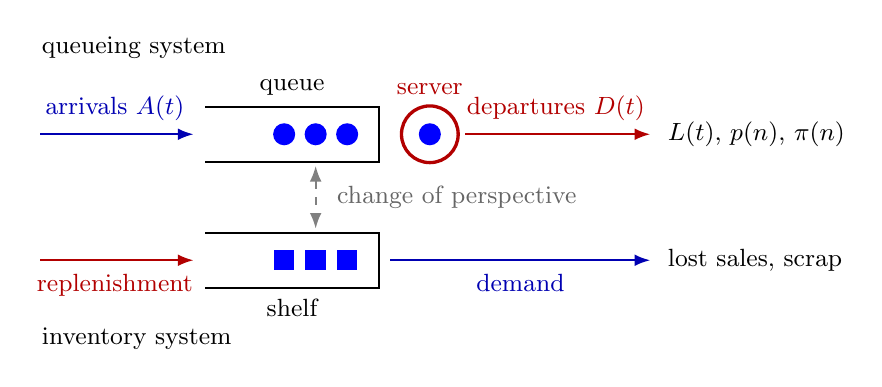
\begin{tikzpicture}[font=\small, >={Latex[length=2mm]}]
  % ---------- queueing system ----------
  \node[anchor=west] at (-0.1,2.7) {queueing system};
  \draw[->, thick, blue!70!black] (0,1.6) -- (1.95,1.6);
  \node[blue!70!black, anchor=south] at (0.95,1.65) {arrivals $A(t)$};
  \draw[thick] (2.1,1.95) -- (4.3,1.95) -- (4.3,1.25) -- (2.1,1.25);
  \foreach \x in {3.1,3.5,3.9} \fill[blue] (\x,1.6) circle (0.14);
  \node[anchor=south] at (3.2,1.97) {queue};
  \draw[very thick, red!70!black] (4.95,1.6) circle (0.36);
  \fill[blue] (4.95,1.6) circle (0.14);
  \node[red!70!black, anchor=south] at (4.95,1.98) {server};
  \draw[->, thick, red!70!black] (5.4,1.6) -- (7.75,1.6);
  \node[red!70!black, anchor=south] at (6.55,1.65) {departures $D(t)$};
  \node[anchor=west] at (7.85,1.6) {$L(t)$, $p(n)$, $\pi(n)$};
  % ---------- inventory system ----------
  \node[anchor=west] at (-0.1,-1.0) {inventory system};
  \draw[->, thick, red!70!black] (0,0) -- (1.95,0);
  \node[red!70!black, anchor=north] at (0.95,-0.05) {replenishment};
  \draw[thick] (2.1,0.35) -- (4.3,0.35) -- (4.3,-0.35) -- (2.1,-0.35);
  \foreach \x in {3.1,3.5,3.9} \fill[blue] (\x-0.13,-0.13) rectangle (\x+0.13,0.13);
  \node[anchor=north] at (3.2,-0.37) {shelf};
  \draw[->, thick, blue!70!black] (4.45,0) -- (7.75,0);
  \node[blue!70!black, anchor=north] at (6.1,-0.05) {demand};
  \node[anchor=west] at (7.85,0) {lost sales, scrap};
  % ---------- change of perspective ----------
  \draw[<->, thick, dashed, gray] (3.5,1.2) -- (3.5,0.4);
  \node[gray!80!black, anchor=west] at (3.65,0.8) {change of perspective};
\end{tikzpicture}
\end{document}
